\documentclass[a4paper, 12pt]{article}
\usepackage[left = 13 mm, top = 15mm, right = 13 mm, bottom = 23mm, bindingoffset = 7mm]{geometry}
\usepackage[T2A,T1]{fontenc}
\usepackage[utf8]{inputenc}
\usepackage[english,russian]{babel}
\usepackage{graphicx}
\usepackage{amssymb, mathtools}
\usepackage{lipsum}
\usepackage{float}
\usepackage{wrapfig}
\usepackage{indentfirst} 

\newcommand{\HRule}{\rule{\linewidth}{0.3mm}}

\newcommand{\LabTitle}{Пассивные электрические цепи}
\begin{document}




\begin{titlepage}
\begin{center}\large
ФГАУ ВПО <<МОСКОВСКИЙ ФИЗИКО-ТЕХНИЧЕСКИЙ УНИВЕРСИТЕТ>>
\begin{figure}[H]
\centering

\includegraphics[width=15cm]{logo.jpg}
\end{figure}
{\Large
Кафедра радиотехники}

\vfill

\hrule
\vspace{0.3cm}

\huge \LabTitle

\vspace{0.3cm}
\hrule


%\noindent\rule{\textwidth}{0.4mm}
%\huge Магнитометр
%\noindent\rule{\textwidth}{0.4mm}


\end{center}

\vfill


\begin{minipage}{0.7\textwidth}
\textbf{Выполнил:}
Корепанов Г.М.

512 группа

\vspace{0.5cm}

\textbf{Преподаватель:}
Филатов Иван Васильевич
\end{minipage}


\vfill
\centering
 Долгопрудный, 2016 г.




\end{titlepage}


\section*{Интегрирующие и дифференцирующие звенья}

\subsection*{Интегрирующая цепочка}
\subsubsection*{АЧХ}
\begin{figure}[H]
\centering
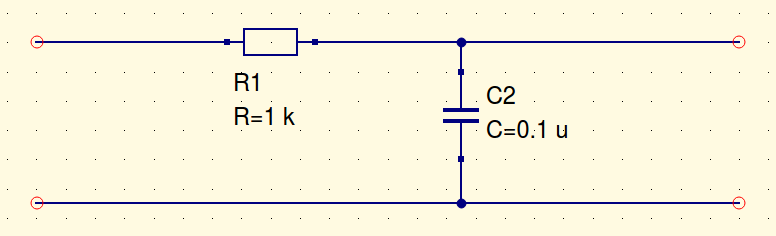
\includegraphics[width=0.8\textwidth]{1-int}
\caption{Интегрирующая цепочка с экспериментальными параметрами}
\end{figure}

Для данной цепочки получаем постоянную времени $\tau = RC \simeq 0,1 $ мс. 

\begin{table}[H]
\centering
\begin{tabular}{|l|l|l|l|l|l|l|l|}
\hline
\textbf{$\mathbf{f/f_0}$} & 0.25 & 0.5  & 1    & 2    & 4    & 8    & 16   \\ \hline
\textbf{K(f)}    & 0.95 & 0.89 & 0.75 & 0.53 & 0.31 & 0.17 & 0.09 \\ \hline
\end{tabular}
\caption{Зависимость коэффициента передачи от частоты, опорная частота $f_0 = 1600$ Гц}
\label{my-label}
\end{table}
\begin{figure}[H]
\centering
% GNUPLOT: LaTeX picture with Postscript
\begingroup
  \fontfamily{sansserif}%
  \selectfont
  \makeatletter
  \providecommand\color[2][]{%
    \GenericError{(gnuplot) \space\space\space\@spaces}{%
      Package color not loaded in conjunction with
      terminal option `colourtext'%
    }{See the gnuplot documentation for explanation.%
    }{Either use 'blacktext' in gnuplot or load the package
      color.sty in LaTeX.}%
    \renewcommand\color[2][]{}%
  }%
  \providecommand\includegraphics[2][]{%
    \GenericError{(gnuplot) \space\space\space\@spaces}{%
      Package graphicx or graphics not loaded%
    }{See the gnuplot documentation for explanation.%
    }{The gnuplot epslatex terminal needs graphicx.sty or graphics.sty.}%
    \renewcommand\includegraphics[2][]{}%
  }%
  \providecommand\rotatebox[2]{#2}%
  \@ifundefined{ifGPcolor}{%
    \newif\ifGPcolor
    \GPcolorfalse
  }{}%
  \@ifundefined{ifGPblacktext}{%
    \newif\ifGPblacktext
    \GPblacktexttrue
  }{}%
  % define a \g@addto@macro without @ in the name:
  \let\gplgaddtomacro\g@addto@macro
  % define empty templates for all commands taking text:
  \gdef\gplbacktext{}%
  \gdef\gplfronttext{}%
  \makeatother
  \ifGPblacktext
    % no textcolor at all
    \def\colorrgb#1{}%
    \def\colorgray#1{}%
  \else
    % gray or color?
    \ifGPcolor
      \def\colorrgb#1{\color[rgb]{#1}}%
      \def\colorgray#1{\color[gray]{#1}}%
      \expandafter\def\csname LTw\endcsname{\color{white}}%
      \expandafter\def\csname LTb\endcsname{\color{black}}%
      \expandafter\def\csname LTa\endcsname{\color{black}}%
      \expandafter\def\csname LT0\endcsname{\color[rgb]{1,0,0}}%
      \expandafter\def\csname LT1\endcsname{\color[rgb]{0,1,0}}%
      \expandafter\def\csname LT2\endcsname{\color[rgb]{0,0,1}}%
      \expandafter\def\csname LT3\endcsname{\color[rgb]{1,0,1}}%
      \expandafter\def\csname LT4\endcsname{\color[rgb]{0,1,1}}%
      \expandafter\def\csname LT5\endcsname{\color[rgb]{1,1,0}}%
      \expandafter\def\csname LT6\endcsname{\color[rgb]{0,0,0}}%
      \expandafter\def\csname LT7\endcsname{\color[rgb]{1,0.3,0}}%
      \expandafter\def\csname LT8\endcsname{\color[rgb]{0.5,0.5,0.5}}%
    \else
      % gray
      \def\colorrgb#1{\color{black}}%
      \def\colorgray#1{\color[gray]{#1}}%
      \expandafter\def\csname LTw\endcsname{\color{white}}%
      \expandafter\def\csname LTb\endcsname{\color{black}}%
      \expandafter\def\csname LTa\endcsname{\color{black}}%
      \expandafter\def\csname LT0\endcsname{\color{black}}%
      \expandafter\def\csname LT1\endcsname{\color{black}}%
      \expandafter\def\csname LT2\endcsname{\color{black}}%
      \expandafter\def\csname LT3\endcsname{\color{black}}%
      \expandafter\def\csname LT4\endcsname{\color{black}}%
      \expandafter\def\csname LT5\endcsname{\color{black}}%
      \expandafter\def\csname LT6\endcsname{\color{black}}%
      \expandafter\def\csname LT7\endcsname{\color{black}}%
      \expandafter\def\csname LT8\endcsname{\color{black}}%
    \fi
  \fi
    \setlength{\unitlength}{0.0500bp}%
    \ifx\gptboxheight\undefined%
      \newlength{\gptboxheight}%
      \newlength{\gptboxwidth}%
      \newsavebox{\gptboxtext}%
    \fi%
    \setlength{\fboxrule}{0.5pt}%
    \setlength{\fboxsep}{1pt}%
\begin{picture}(9354.00,6802.00)%
    \gplgaddtomacro\gplbacktext{%
      \csname LTb\endcsname%
      \put(660,1408){\makebox(0,0)[r]{\strut{}$0$}}%
      \csname LTb\endcsname%
      \put(660,2381){\makebox(0,0)[r]{\strut{}$0.2$}}%
      \csname LTb\endcsname%
      \put(660,3354){\makebox(0,0)[r]{\strut{}$0.4$}}%
      \csname LTb\endcsname%
      \put(660,4327){\makebox(0,0)[r]{\strut{}$0.6$}}%
      \csname LTb\endcsname%
      \put(660,5300){\makebox(0,0)[r]{\strut{}$0.8$}}%
      \csname LTb\endcsname%
      \put(660,6273){\makebox(0,0)[r]{\strut{}$1$}}%
      \csname LTb\endcsname%
      \put(924,968){\makebox(0,0){\strut{}$0$}}%
      \csname LTb\endcsname%
      \put(1974,968){\makebox(0,0){\strut{}$2$}}%
      \csname LTb\endcsname%
      \put(3025,968){\makebox(0,0){\strut{}$4$}}%
      \csname LTb\endcsname%
      \put(4075,968){\makebox(0,0){\strut{}$6$}}%
      \csname LTb\endcsname%
      \put(5125,968){\makebox(0,0){\strut{}$8$}}%
      \csname LTb\endcsname%
      \put(6175,968){\makebox(0,0){\strut{}$10$}}%
      \csname LTb\endcsname%
      \put(7226,968){\makebox(0,0){\strut{}$12$}}%
      \csname LTb\endcsname%
      \put(8276,968){\makebox(0,0){\strut{}$14$}}%
      \csname LTb\endcsname%
      \put(9326,968){\makebox(0,0){\strut{}$16$}}%
    }%
    \gplgaddtomacro\gplfronttext{%
      \csname LTb\endcsname%
      \put(-9,3840){\rotatebox{-270}{\makebox(0,0){\strut{}$K(f)$}}}%
      \put(5125,308){\makebox(0,0){\strut{}$f/f_0$}}%
    }%
    \gplbacktext
    \put(0,0){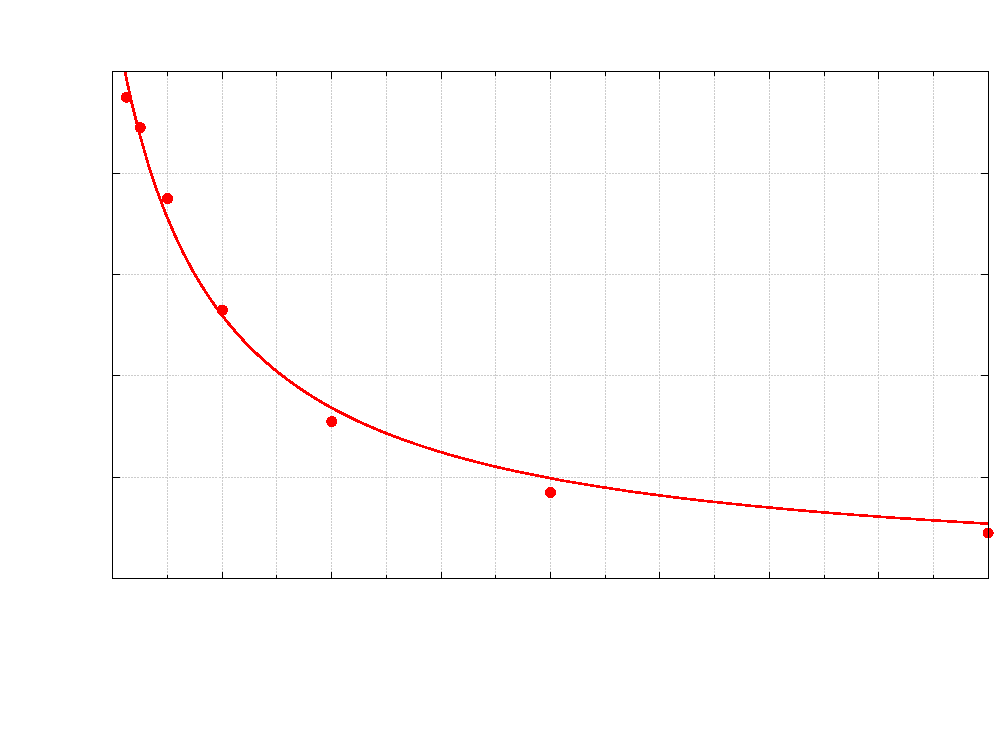
\includegraphics{1intplot}}%
    \gplfronttext
  \end{picture}%
\endgroup

\caption{Амплитудно-частотная характеристика}
\end{figure}

\begin{figure}[H]
\centering
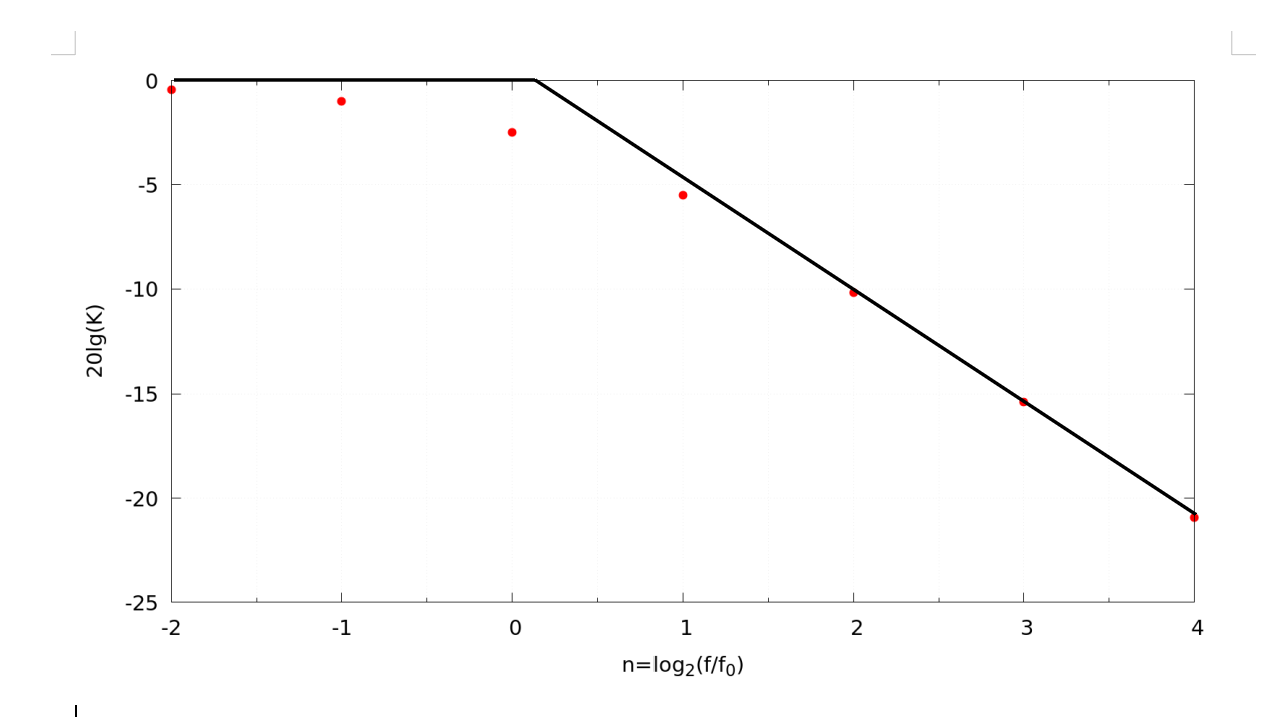
\includegraphics[width=1\textwidth]{bodeint}
\caption{Соответсутвующий граф Боде}
\end{figure}


По графикам оцениваем граничную частоту:
$$f_{\text{гр}} = 1680 \text{ Гц},$$
 что практически совпадает с теоретической $f_0 = \frac{1}{2\pi RC} = 1600$ Гц.
 
\subsubsection*{Постоянная времени}
\begin{figure}[H]
\centering
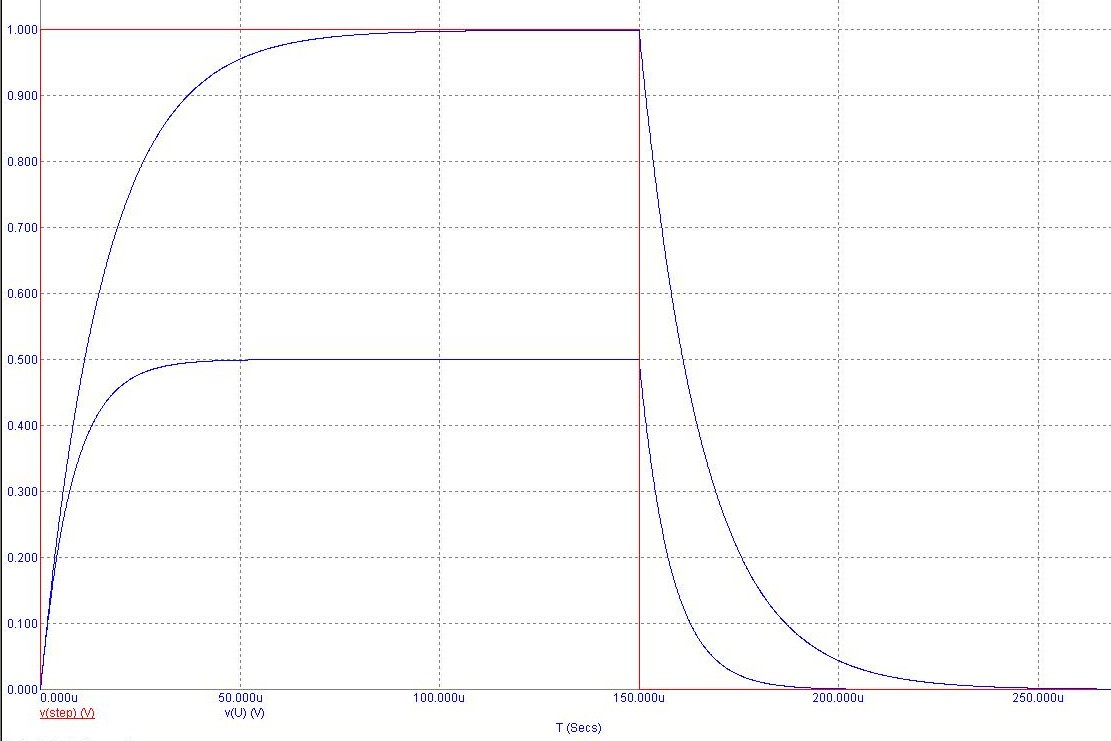
\includegraphics[width=0.8\textwidth]{inttau}
\caption{Иллюстрация к определению постоянной времени}
\end{figure}

В случае интегрирующей цепочки постоянная времени равна времени нарастания фронта до уровня $1-1/e$. По осциллограмме находим $\tau = 0,085$ мс. Проверяем сходимость результатов:

$$\frac{1}{2\pi \tau} \simeq 1872 \text{ Гц} $$,
отлично сходится с предыдущими измерениями (при данной точности эксперимента).
\subsection*{Дифференцирущая цепочка}

Выполняя все действия по аналогии, получаем значения
$$f_0 = 1765 \text{ Гц},$$
$$\tau = 0,091 \text{ мс}.$$

Из-за того, что напряжение в данном случае снимается с резистора, график переходной характеристики (отклик на воздействие -- функцию Хевисайда) <<инвертируется>>, и поэтому в данном случае $\tau$ - время спада вершины импульса до уровня $1/e$.
\begin{figure}[H]
\centering
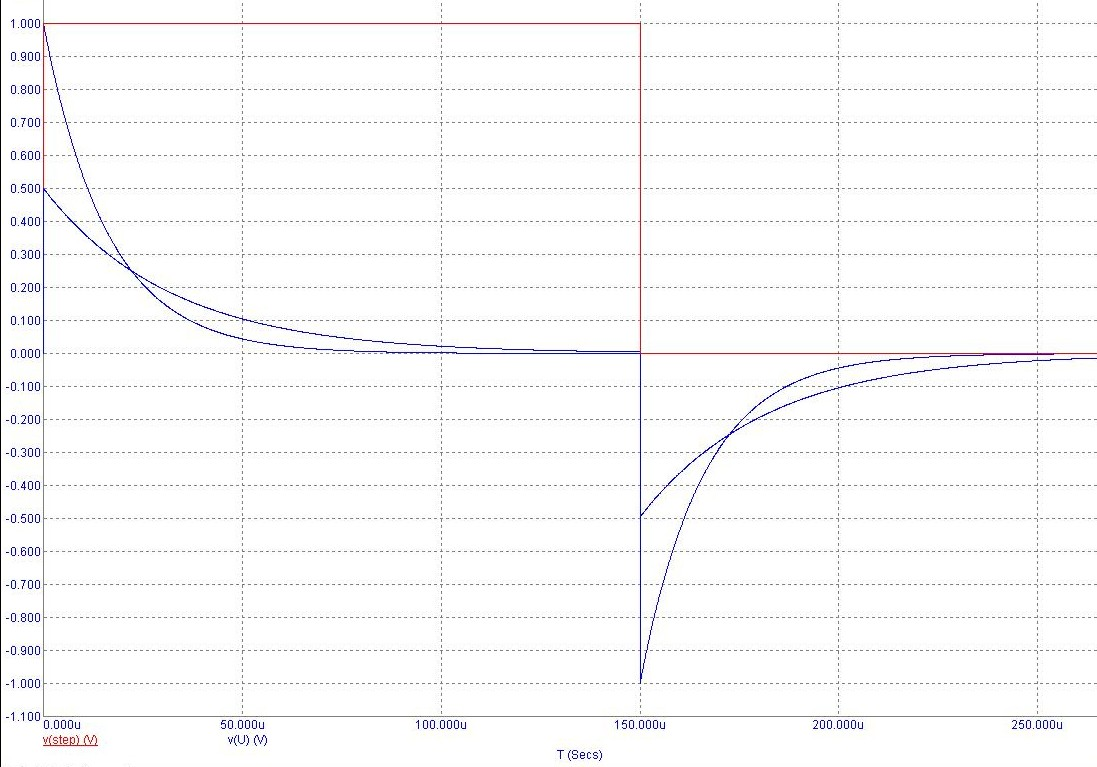
\includegraphics[width=0.8\textwidth]{difftau}
\caption{Иллюстрация к определению постоянной времени}
\end{figure}

\subsection*{MicroCap -- интегрирующая цепочка}
\begin{figure}[H]
\centering
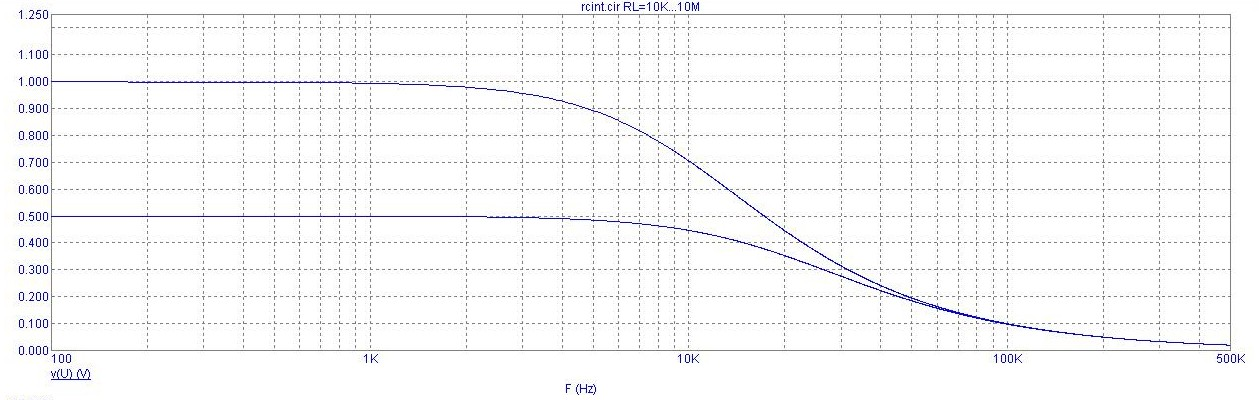
\includegraphics[width=1\textwidth]{rcintanal}
\caption{Иллюстрация к определению верхней частоты}
\end{figure}

Из графика частотной харакетристики получаем граничную частоту $f_\text{гр} = 10$ кГц, что хорошо сходится со значением, посчитанным по формуле $\frac{1}{2\pi \tau}$.
Из графика для переходной характеристики получаем $\tau_{\text{эксп}} = 15,88$ мкс.
\subsection*{MicroCap -- дифференцирующая цепочка}
Повторяем все действия. получаем граничную частоту $f_\text{гр} = 10$ кГц, постоянную времени $\tau_{\text{эксп}} = 16$ мкс.

На этот раз частотные характеристики <<переворачиваются>>:
\begin{figure}[H]
\centering
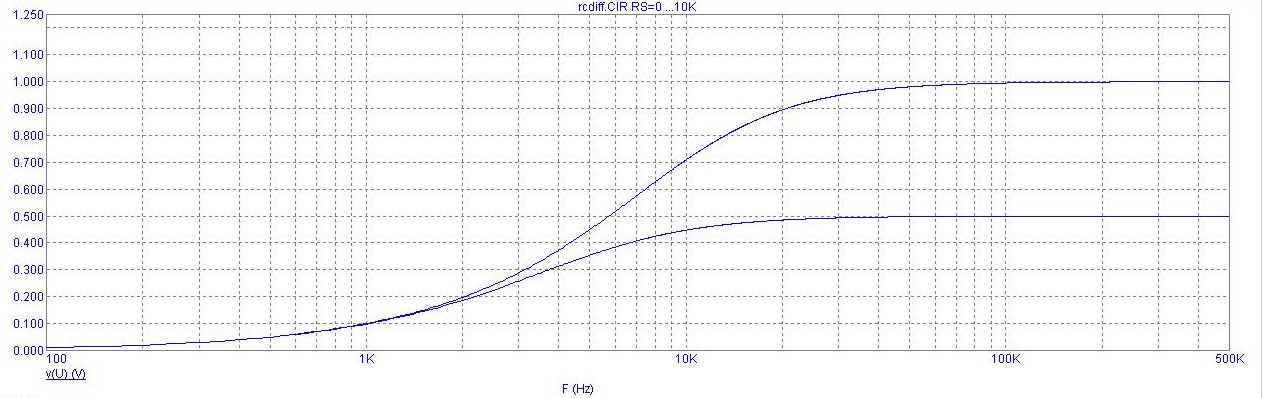
\includegraphics[width=1\textwidth]{rcdiffanal}
\caption{Иллюстрация к определению нижней частоты}
\end{figure}

\subsection*{MicroCap -- распредление мощностей}
На граничной частоте активная и рективная мощности, вы деляющиеся в схеме, равны по модулю и противоположны по знаку:
\begin{figure}[H]
\centering
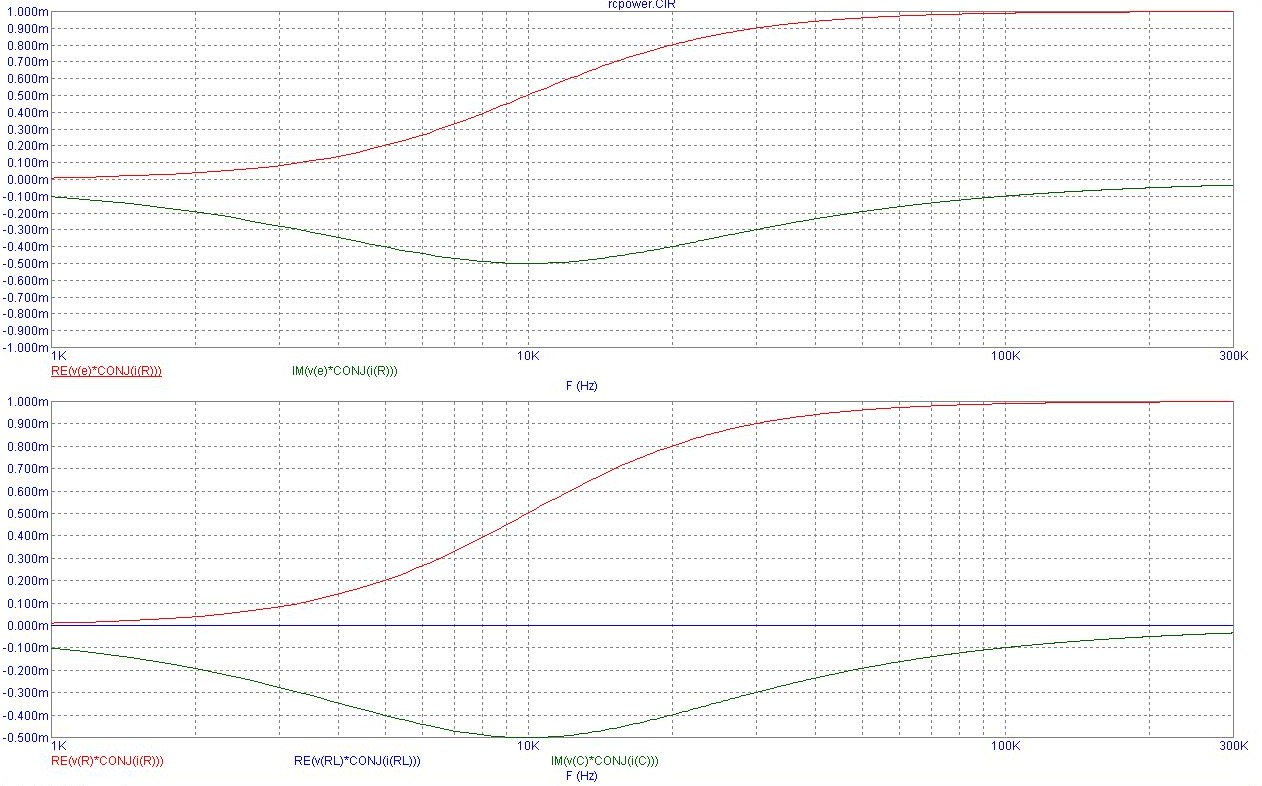
\includegraphics[width=1\textwidth]{rcpowe}
\caption{Закон сложения мощностей}
\end{figure}

\section*{RC-звенья второго порядка}
\begin{figure}[H]
\centering
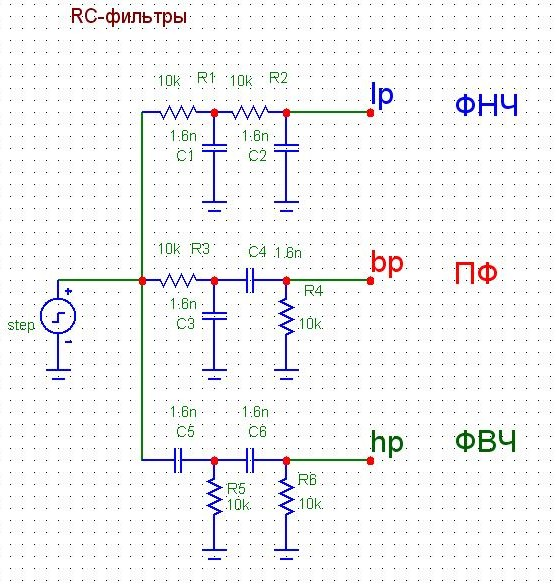
\includegraphics[width=0.6\textwidth]{rcpole}
\caption{Схема изучения звеньев второго порядка}
\end{figure}

$$f_0 = \frac{1}{2\pi RC} = 9947 \text{ Гц}.$$
На частоте $f_0$ для всех трех фильтров затухание одинаково и равно $K = -9,5\ dB$.
\subsection*{Скорость нарастания затухания:}
\textbf{ФНЧ}: $40dB/$дек, \textbf{ПФ}: $20dB/$дек, \textbf{ФВЧ}: $40dB/$дек.
\subsection*{Сдвиг фаз на разных частотах}
\begin{table}[H]
\centering
\begin{tabular}{|l|l|l|l|}
\hline
$\omega$     & $0$         & $f_0$       & $\infty$      \\ \hline
\textbf{ФНЧ} & $0^{\circ}$ & $-90^{\circ}$ & $-180^{\circ}$ \\ \hline
\textbf{ПФ}  & $90^{\circ}$ & $0^{\circ}$ & $-90^{\circ}$ \\ \hline
\textbf{ФВЧ} & $180^{\circ}$ & $90^{\circ}$ & $0^{\circ}$ \\ \hline
\end{tabular}
\caption{Сдвиги фаз}
\end{table}

Двусторонняя полоса пропускания между точками со сдвигом фаз $\pm \pi/4$:
$$\Delta f = 29 \text{ кГц} \simeq 3f_0.$$
\begin{figure}[H]
\centering
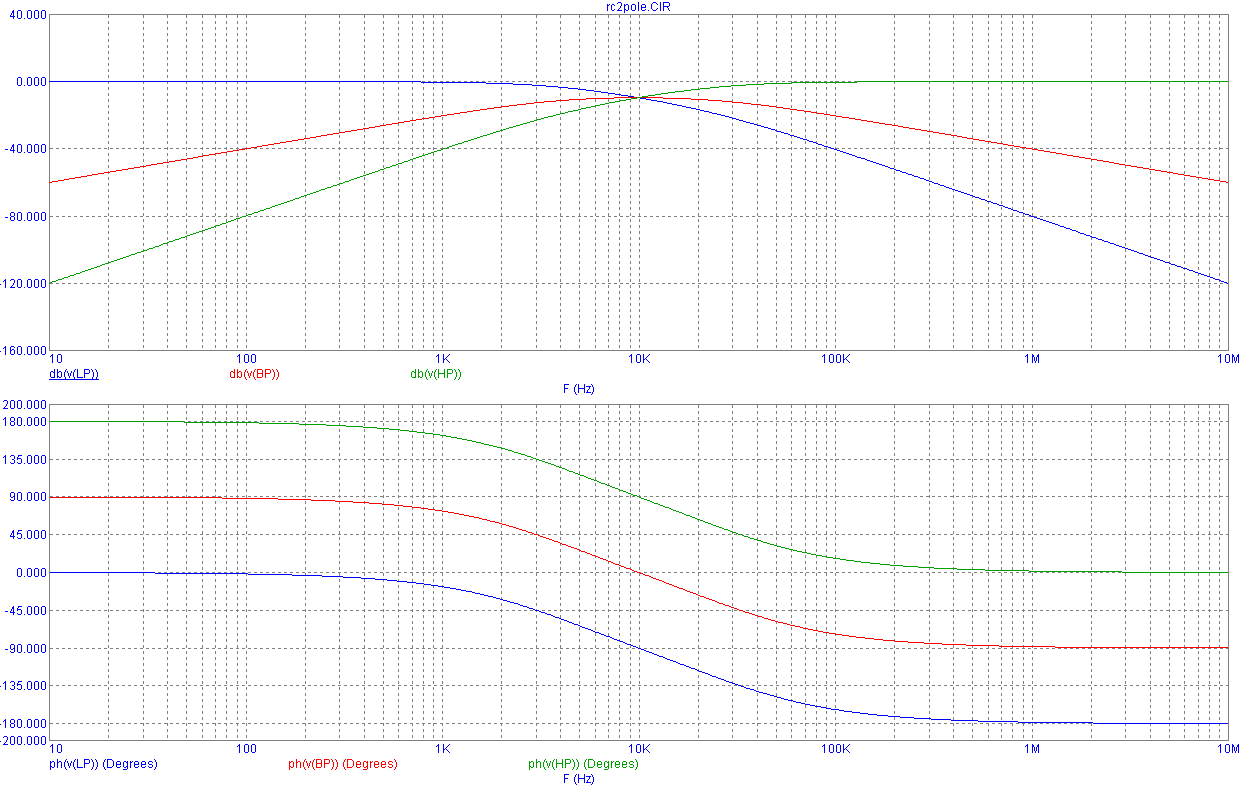
\includegraphics[width=1\textwidth]{rcpoleanal}
\caption{Анализ звеньев второго порядка}
\end{figure}

\subsection*{Переходная характеристика}
Время спада выброса до уровня $1/e$: $\tau_{-} = 4,9$ мкс (ФВЧ); время нарастания фронта до уровня $1-1/e$: $\tau_{+} = 48$ мкс (ФНЧ).

$$\tau_+ / \tau_- \simeq 10.$$
\begin{figure}[H]
\centering
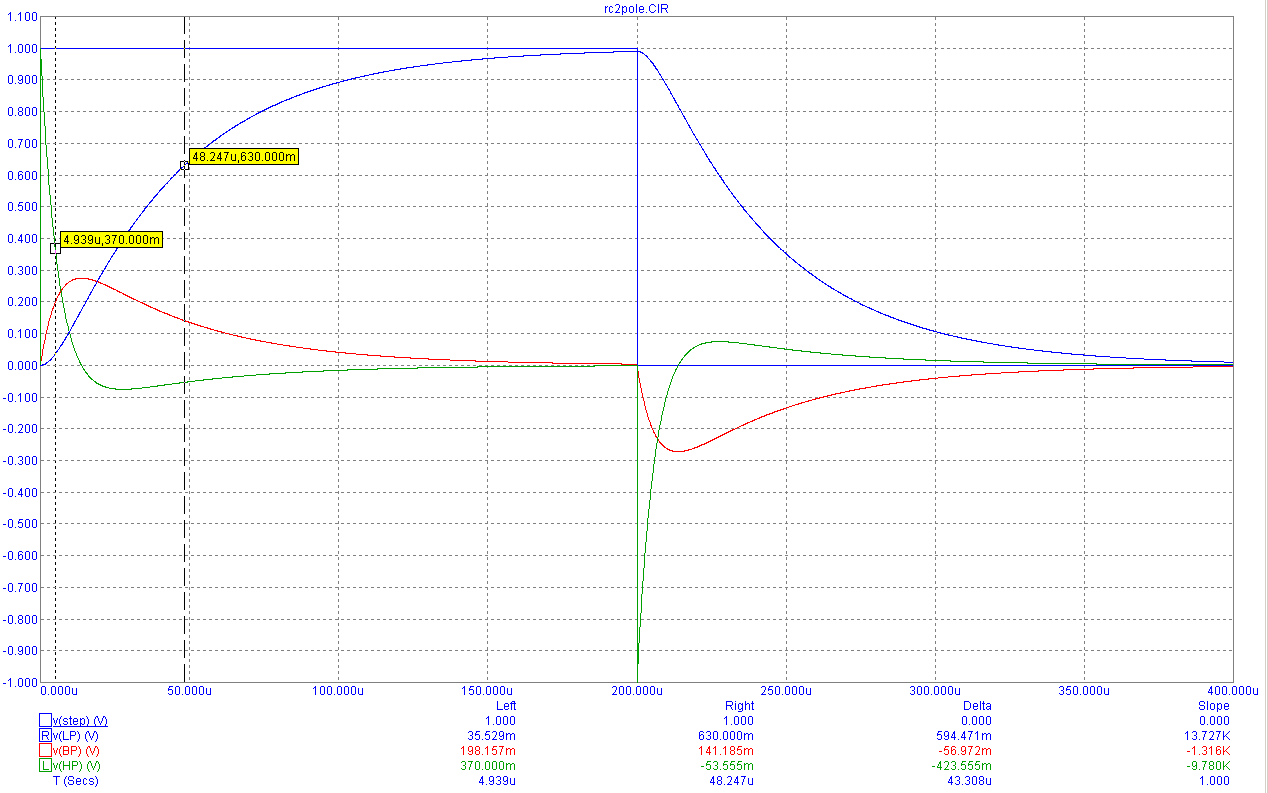
\includegraphics[width=1\textwidth]{rcpoletran}
\caption{Анализ звеньев второго порядка -- переходная характеристика}
\end{figure}

\section*{Фазовращатели}
Наибольший диапазон перестройки фазы $\Delta \varphi = 121^\circ$ при $f=25$ кГц:
\begin{figure}[H]
\centering
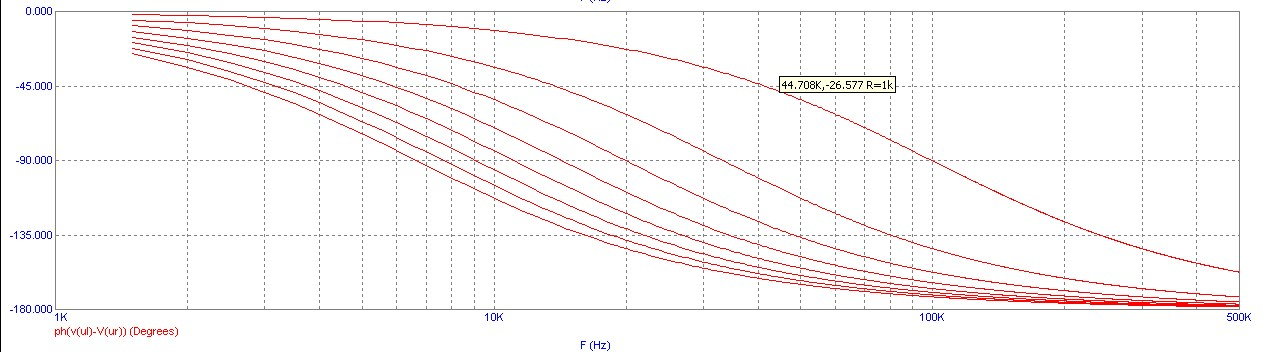
\includegraphics[width=1\textwidth]{phsshift}
\caption{Фазовращатель}
\end{figure}

\subsection*{Двойной Т-образный мост}
\begin{figure}[H]
\centering
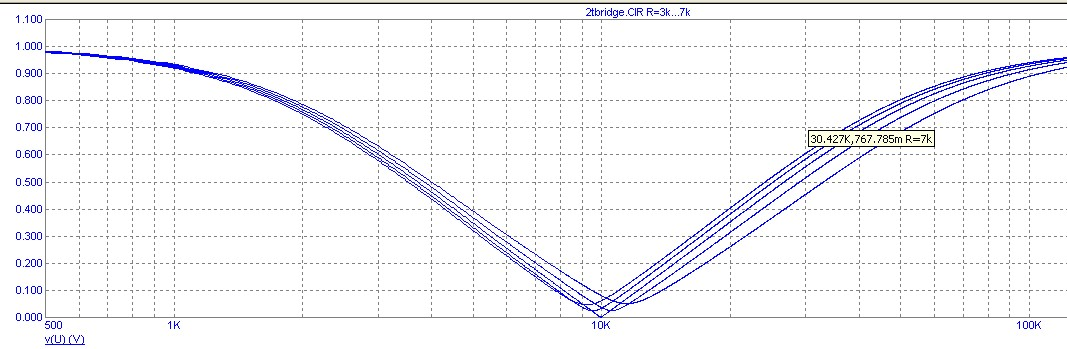
\includegraphics[width=1\textwidth]{2tbridge}
\caption{К измерению ширины полосы режекции}
\end{figure}
Ширина полосы режекции по уровню $-3\ dB$ равна $\Delta f = 39$ кГц. $\Delta f  \simeq 4f_0$.

\subsection*{Переходная характеристика}
Время спада первого пика до уровня $1/e$: $\tau_{+} = 4$ мкс; время нарастания вершины до уровня $1-1/e$: $\tau_{+} = 55$ мкс. Теоретические значения: $\tau_+ = 4,2$ мкс, $\tau_- = 59$ мкс, что хорошо согласуется с экспериментом.
\begin{figure}[H]
\centering
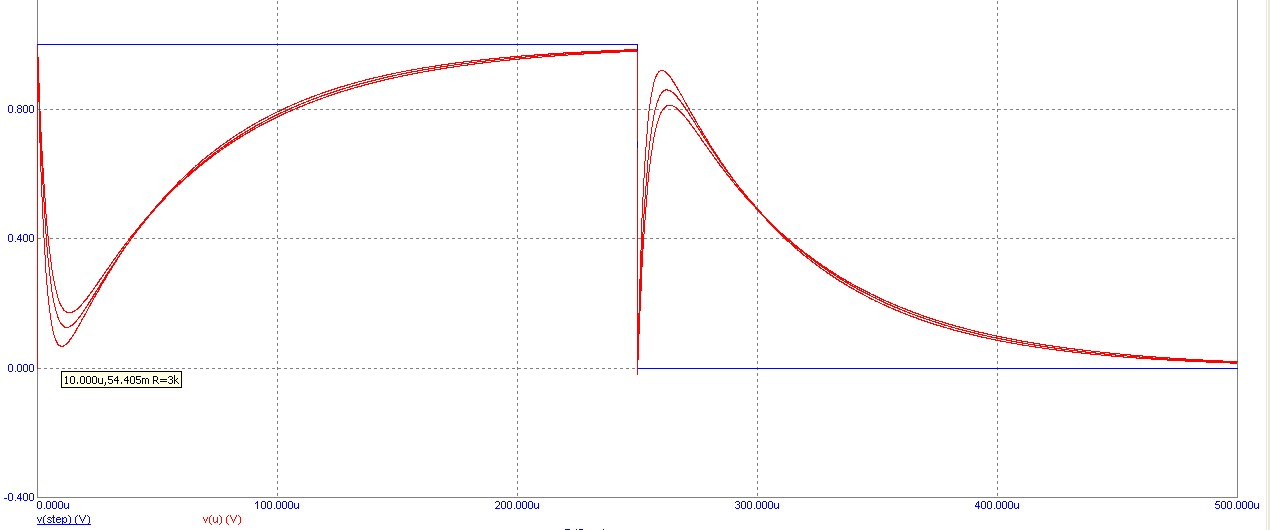
\includegraphics[width=1\textwidth]{2tbridgetran}
\caption{Степпинг переходной харатеристики, $R = [3k,7k|2k]$}
\end{figure}
\subsection*{Частоты и добротности нулей передачи при разных R}
Определим добротности нулей передачи, измеряя полосы $\Delta f$ по интервалам изменения фазы на $\pm \pi/4$:

\begin{table}[H]
\centering
\begin{tabular}{|l|l|l|l|}
\hline
\textbf{$R$}            & $4,9k$ & $5,0k$   & $5,1k$ \\ \hline
\textbf{$\Delta f$, Гц} & 51     & 0        & 50     \\ \hline
\textbf{$Q$}            & 200    & $\infty$ & 200    \\ \hline
\textbf{$f_0$, Гц}      & 10048  & 9997     & 9948   \\ \hline
\end{tabular}
\caption{Добротности нулей передачи}
\label{my-label}
\end{table}

\section*{Последовательный резонанс}
Соберём полосовой фильтр с параметрами $C=1000$ пФ, $L = 220$ мкГн, $ r = 91$ Ом:
\begin{figure}[H]
\centering
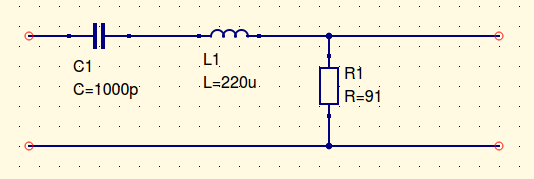
\includegraphics[width=0.6\textwidth]{polfil}
\caption{Схема полосовго фильтра}
\end{figure}
Резонансная частота:
$$f_\text{теор} = \frac{1}{2\pi \sqrt{LC}} = 340 \text{ кГц},$$
$$f_\text{эксп} = 376 \text{ кГц}.$$
Коэффициент предачи на резонансной частоте $K(f_0) = \frac{U_\text{вых}}{U_\text{вх}} = 0,86$
Ширина пика по уровню $-3\ dB$:
$$\Delta f = |309 \text{ кГц} - 441 \text{ кГц}| = 132 \text{ кГц}$$
$$Q_\text{теор} = \frac{1}{r}\sqrt{\frac{L}{C}} = 5,15$$
$$Q_\text{эксп} = \frac{f_0}{\Delta f} = 2,8$$
Расхождение, очевидно, вызвано неучтённым сопротивлением катушки и проводов.
\subsection*{Переходная характеристика}
\begin{figure}[H]
\centering
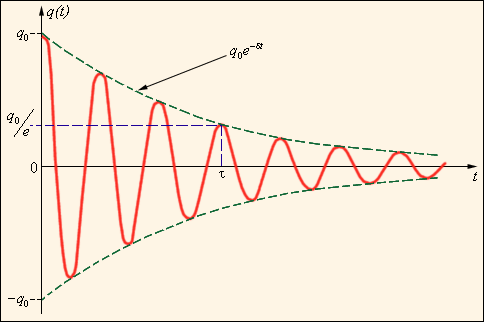
\includegraphics[width=0.6\textwidth]{tranzat}
\caption{переходная характеристика резонансной цепочки}
\end{figure}
Время затухания до уровня $1/e$: $\tau = 2,9$ мкс. Период колебаний $T = 2,9$ мкс.
$$\tau = \frac{2L}{R} = \frac{QT}{\pi} \rightarrow Q = \frac{\pi \tau}{T} \simeq 3,$$
$$f_0 = 1/T \simeq 344 \text{ кГц}$$
Как видим, и таким методом получаем отличное схождение с экспериментом.

\section*{Изучение резонансных цепочек в MicroCap}
Графики и зависимости, полученные теоретически в программе моделированием, отлично сходятся с экспериментами, поставленными выше на реальных цепях. 
\subsection*{Зависимость групповых хадержек полосового фильтра от R}

\begin{table}[H]
\centering
\begin{tabular}{|l|l|}
\hline
\textbf{$R$, Ом} & \textbf{$\tau_g$, мс} \\ \hline
10               & 444                   \\ \hline
20               & 277                   \\ \hline
40               & 156                   \\ \hline
100              & 64                    \\ \hline
\end{tabular}
\caption{Групповые задержки}
\label{my-label}
\end{table}

Получаем хорошую сходимость с теоретической формулой, которая легко модет быть получена из определения групповой задержки:

$$\tau_g = -\frac{d\varphi}{d\omega} = \frac{Q}{\pi f_0}$$

\section*{Выводы}
Были получены навыки работы с простейшими электричискими цепями, изучены основные методы обработки сигналов, коэффициентов передачи и прочих характеристик линейных цепей. Изучены основные понятия электротехники. 
\end{document}


